
\section{ Relief Generation}

In Chinese paintings, each brushstroke is often introduced to depict something specific in the real world.
Thus, the output of our stroke-based decomposition of these paintings is a set of graphical objects that are meaningful with regard to the set of real objects the paintings depict. It is natural to generate depth information from brushstrokes,here,we present a relief generation method based brushstrokes  \cite{xu2006animating} . \\


\subsection{comparison}

Previous work focused on relief generation from images are mainly based on photos.The method proposed in \cite{yeh2017interactive} was design for reconstruct high-relief 3D models from a single input image of organic objects with nontrivial shape profile. \\
Our high relief generation result is similar to Yeh et al.'s method, with the difference being that we replace the manual segmented regions on image with our extracted brushstroke regions on each layer and combine the SFS with inflation, finally ,we re-render the high-relief with every correspond brush stroke texture. \\
%we compare our results with the most closely-related recent work \cite{yeh2017interactive}. In particular, we compare the visual plausibility of the results, with large rotations from the original viewing direction (please refer to the supplementary video, available online, for animated versions of the comparison). 
Following with our method, we compare our results with  \cite{yeh2017interactive}'s method at three aspects: segmentation, local layering, and inflation.\\
\textbf{Segmentation:} \\
As a comparison, our results can preserve the thin and complex shapes of brushstrokes,as showing in Fig.\ref{fig:vsmsergrab}. \\ 
\begin{figure}[h]
	\centering % avoid the use of \begin{center}...\end{center} and use \centering instead (more compact)
	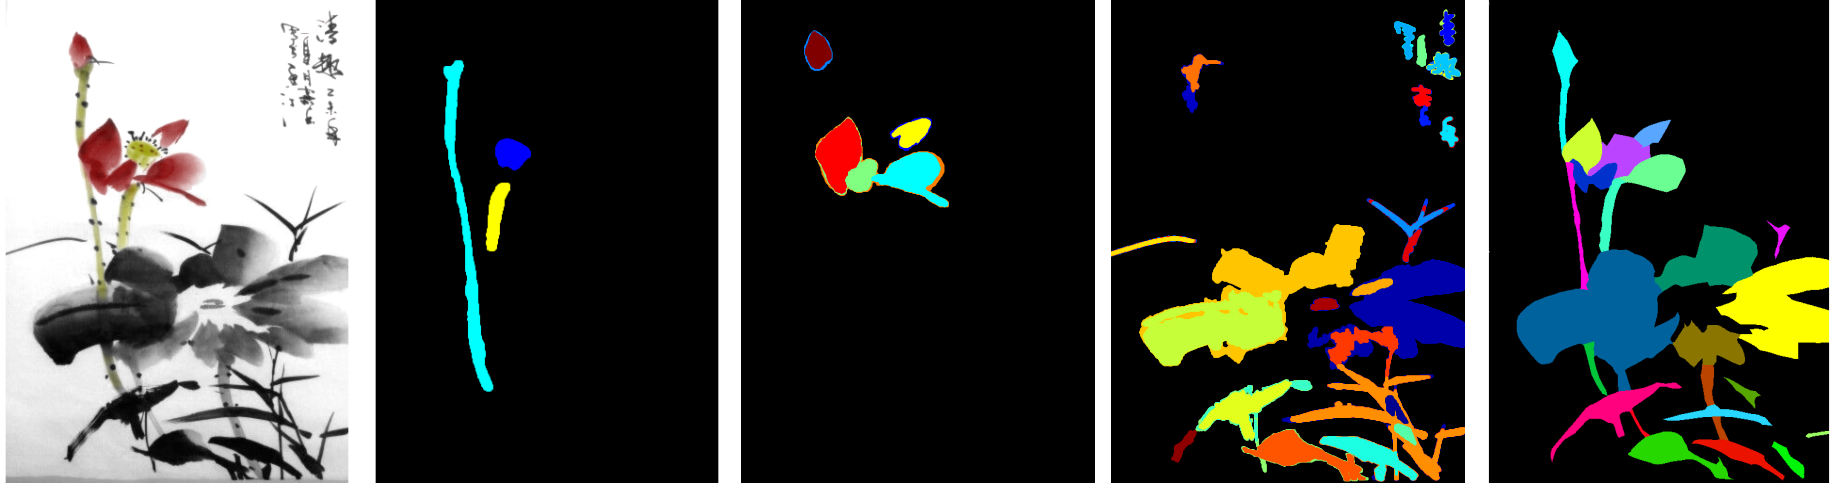
\includegraphics[width=\columnwidth]{vsmsergrab}
	\caption{00 }
	\label{fig:vsmsergrab}
\end{figure}\\
\textbf{Inflation: }\\
Yeh et al's method is mainly designed for reconstructing smooth and organic shapes, where the inflation model assumes smooth surfaces.
While in our algorithm, we use opacity to generate the bas-relief, and we apply the displacement map to the high relief, which maintains the details of brush strokes better, see Figure .\\
Figure  demonstrate the difference between applying 
To preserve the richness of fine details on brush strokes,    
The overall impression is quite ok but not as pleasing as the one achieved with our approach.
Note the problems at the left foot in the spatial result and compare the richness of fine details of on the wings, the torch and also the fingers in the two results\\
\textbf{Local layering:} \\
Each brushstroke covers a region on the canvas and they may overlap with each other, some quite heavily in a painting. In our method, overlapped brushstroke with different colors are separated into different layers. 

GrabCut was performed on the red pigment for the top painting, and on the black pigment for the bottom painting.  
\cite{yeh2017interactive} determines and categorize the local layering, or depth ordering between segmented regions by employ the hypotheses in \cite{yeh20152},\cite{liu2013stereoscopizing}, i.e., T-junctions and overlap area, to construct the layering information. In order faithfully complete the overlap area, it requires clear edge of region to form the T-junctions while the brush stroke ma
To make sure the information is retained,   While we maintained such feature,  Figure demonstrate the difference between Yeh  \\
In  which clearly shows improved localization of  painted objects in the black rectangular regions.

\textbf{Transparency: }\\
To maintain the opacity of brushstrokes we 
In \cite{yeh2017interactive}' method, it is noteworthy that our method preserve the opacity ,see Fig , \\ 


\textbf{Hierarchical structure: }\\
Our algorithm uses hierarchical regions to represents the brush strokes, in contrast to previous work [Tan et al. 2016] which solves a similar problem using inpainting method. Intuitively, we would expect that our model would be able to reconstruct paintings into high relief which maintains such feature, and the experiment we show in Fig. 8 confirms that. 

particularly,for some area like feather and , where coarse to fine structure painting skill is applied. We found that the stroke based high relief generation could better preserve such feature . 

 


